%!TEX root = ../Thesis.tex
\label{chap:pil}
\section{Design}
\label{sect:expdes}
The goal of this pilot study is three-folded. The first one being crowdsourcing annotations on premise-hypothesis pairs to answer the four research questions introduced in Chapter \ref{chap:intr} and which are repeated below:\\

\begin{enumerate}[RQ1.-]
        \item In a complex sentence like examples (\ref{ex:moodaltind}) and (\ref{ex:moodaltsbjv}), how does the mood alternation of the embedded verb that occurs due to the negation of the main or matrix verb affect the factuality value of the embedded event?\label{rq1}
        \item In a simple sentence like examples (\ref{ex:moodaltindadv2}) and (\ref{ex:moodaltsbjvadv2}), how does the mood alternation caused by an adverb of doubt or possibility affect the factuality judgment of the event?\label{rq2}
        \item How does an individual subject, like the one in example (\ref{ex:moodaltindadv2}), affect the factuality judgment of the event?\label{rq3}%
        \item How does a subject that refers to a collective entity like \textit{the government}, affect the factuality judgment of the event?\label{rq4}%
\end{enumerate} 

These questions yield the four experimental conditions: negation (\ref{rq1}) and with examples (\ref{ex:negbas}) to (\ref{ex:negsub}) , adverb or possibility (\ref{rq2}) and exemplified in (\ref{ex:posbas}) to (\ref{ex:possub}), individual (\ref{rq3}) and shown in (\ref{ex:negbas}) to (\ref{ex:negsub}), and collective (\ref{rq4}) presented in (\ref{ex:posbas}) to (\ref{ex:possub}). Furthermore, given the novelty of these conditions and to ensure experimental soundness, the second and third goals of the study are to ensure the correctness of the experimental design and procedure, and to explore different possibilities of statistical analysis, so that in the final study the data is properly analyzed and represented.\\

\begin{exe}
  \ex{\gll El hijo oyó que le estaban llamando.\\ the.\M.\Sg{} son.\M.\Sg{} hear.\Pst.\Pfv.\Ind.\Tsg{} that him be.\Pst.\Ipfv.\Ind.\Tpl{} call.\Ger{} \\\glt The son heard that they were calling him.}\label{ex:negbas}
  \ex{\gll El hijo de la actriz no oyó que le estaban llamando.\\ the.\M.\Sg{} son.\M.\Sg{} of the.\F.\Sg{} actress.\F.\Sg{} not hear.\Pst.\Pfv.\Ind.\Tsg{} that him be.\Pst.\Ipfv.\Ind.\Tpl{} call.\Ger{} \\\glt The actress' son didn't hear that they were calling him.}\label{ex:negind}
 \ex{\gll El hijo de Nicole Kidman no oyó que le estuvieran llamando.\\ the.\M.\Sg{} son.\M.\Sg{} of Nicole Kidman not hear.\Pst.\Pfv.\Ind.\Tsg{} that him be.\Pst.\Ipfv.\Sbjv.\Tpl{} call.\Ger{} \\\glt Nicole Kidman's son didn't hear that they were calling him.}\label{ex:negsub}
\end{exe}

If we take the four conditions, sort them into two groups, mood alternation for negation and adverb, specificity for individual and collective; and cross them, we obtain a 2x2 design, where each conditon is divided into 3 subconditions or categories. The negation and adverb conditions are divided into three categories: baseline (B) shown in examples (\ref{ex:negbas}) and (\ref{ex:posbas}), where there is no negation of the matrix verb or presence of a doubt or possibility adverb; indicative (I), portrayed in examples (\ref{ex:negind}) and (\ref{ex:posind}), where we have a mood induced adverb and the verb is in indicative mood; and subjunctive (S), exemplified in (\ref{ex:negsub}) and (\ref{ex:possub}), where we have a mood induced adverb and the verb is in subjunctive mood.\\ 

The specificity conditions are also divided into three categories: common (C), where the subject is a common noun with the determiner as its only complement as in examples (\ref{ex:negbas}) and (\ref{ex:posbas}); mixed (M), where the subject is a common noun but with a determiner and another complement like examples (\ref{ex:negind}) and (\ref{ex:posind}); and proper (P), where the subject is directly a proper noun like example (\ref{ex:possub}) or there is a relation to a proper noun, like in example (\ref{ex:negsub}).\\

\begin{exe}
  \ex{\gll El sindicato tenía otra idea.\\ the.\M.\Sg{} union.\M.\Sg{} have.\Pst.\Pfv.\Ind.\Tsg{} another.\F.\Sg{}/a.different idea.\F.\Sg{} \\\glt The union had another/a different idea.}\label{ex:posbas}
  \ex{\gll Quizás el sindicato de la empresa tenía otra idea.\\ maybe the.\M.\Sg{} union.\M.\Sg{} from the.\F.\Sg{} company.\F.\Sg{} have.\Pst.\Pfv.\Ind.\Tsg{} another.\F.\Sg{}/a.different idea.\F.\Sg{} \\\glt Maybe the company's union had another/a different idea.}\label{ex:posind}
  \ex{\gll Quizás Comisiones Obreras tuviera otra idea.\\ maybe Comisiones Obreras have.\Pst.\Pfv.\Sbjv.\Tsg{} another.\F.\Sg{}/a.different idea.\F.\Sg{} \\\glt Maybe Comisiones Obreras had another/a different idea.}\label{ex:possub}
\end{exe}

As to the set of labels used to annotate each pair, as in \citet{de2012did} the labels from \citet{sauri2009factbank} minus \textit{certain but unknown output} (CTu) were used. But since, as mentioned in the previous chapter, the acceptability of sentences like (\ref{ex:moodaltindadv2}), where we have a nominal phrase between the adverb of possibility and the verb, was not certain, another label, \textit{not a sentence} (NaS), was added resulting in the following set of 8 labels, represented for simplicity as a one-dimension scale in Figure \ref{fig:labels}: certainly yes (CT+), probably yes (PR+), possibly yes (PS+), unknown or uncommitted (Uu), possibly not (PS-), probably not (PR-), certainly not (CT-), not a sentence (NaS).\\

\begin{figure}
\centering
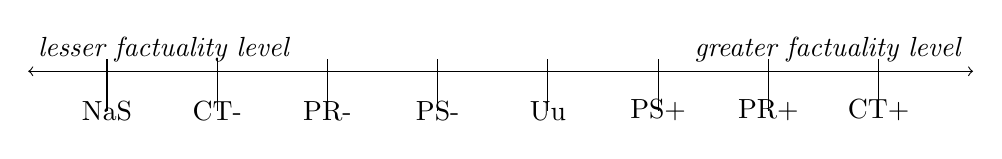
\begin{tikzpicture}
\draw[<->] (-1,0) node[anchor=south west]{\textit{lesser factuality level}}-- (11,0) node[anchor=south east]{\textit{greater factuality level}};
\draw (0,0.15) -- (0,-0.5) node[anchor=center]{NaS};
\draw (1.4,0.15) -- (1.4,-0.5) node[anchor=center]{CT-};
\draw (2.8,0.15) -- (2.8,-0.5) node[anchor=center]{PR-};
\draw (4.2,0.15) -- (4.2,-0.5) node[anchor=center]{PS-};
\draw (5.6,0.15) -- (5.6,-0.5) node[anchor=center]{Uu};
\draw (7,0.15) -- (7,-0.5) node[anchor=center]{PS+};
\draw (8.4,0.15) -- (8.4,-0.5) node[anchor=center]{PR+};
\draw (9.8,0.15) -- (9.8,-0.5) node[anchor=center]{CT+};
\end{tikzpicture} 
\caption[Ordered labels for the pilot study.]{Ordered representation of the labels used for annotating the corpus. Each label stands for: certainly yes (CT+), probably yes (PR+), possibly yes (PS+), unknown or uncommitted (Uu), possibly not (PS-), probably not (PR-), certainly not (CT-), not a sentence (NaS).}\label{fig:labels}
\end{figure}


\begin{table}[h!]
\centering
\begin{tabular}{|c|c|c|c|c|c|}
\hline
\multicolumn{6}{|c|}{Data Generation within Experimental Design I}\\\hline
                      & & &\multicolumn{3}{c|}{SPECIFICITY} \\\cline{4-6} 
                      & & & \multicolumn{3}{c|}{Individual}\\\cline{4-6} 
                      & & & C & M & P\\\hline 
\multirow{6}{*}{MOOD} & \multirow{3}{*}{Negation} & B & S1 & V1 &V1\\\cline{3-6}
                      &                           & I & V1 & V1 &V1\\\cline{3-6}
                      &                           & S & V1  &V1 &V1\\ \cline{2-6}\cline{2-6}                     
                      &\multirow{3}{*}{Possibility}& B & S3 &V3& V3 \\\cline{3-6}
                      &                           & I & V3 & V3 & V3\\\cline{3-6}
                      &                           & S & V3 & V3 & V3*\\\hline                                                          
\end{tabular}
\caption[Experimental conditions and corpus generation I.]{Experimental conditions and corpus generation first part. Each cell is for 9 pairs. \textbf{S} followed by a number stands for set of seeds, \textbf{V} stands for variants, with the number indicating the corresponding set of seeds. \textbf{*} indicates where the 2 mistaken pairs are. \textbf{B, I, S} stands for \textit{baseline, indicative, subjunctive}, and \textbf{C, M, P} stands for \textit{common, mixed, proper}.}
\label{tab:datagen1}
\end{table}

\section{Dataset}
As to the dataset to be annotated, it was constructed by first writing 9 seed premises for each of the four baseline-common combinations and from them the hypotheses were extracted to form the pairs. Then these seeds were changed across conditions, yielding a total of 324 premise-hypothesis pairs\footnote{Upon reviewing the pairs after the experiment was run, it was noticed that there was a mistake on 2 of them, thus yielding them invalid. The whole two seeds were taken out for analysis, yielding a total of 306 analysed pairs.}. Tables \ref{tab:datagen1} and \ref{tab:datagen2} show this generation process together with the experimental design.\\

\begin{table}[h!]
\centering
\begin{tabular}{|c|c|c|c|c|c|}
\hline
\multicolumn{6}{|c|}{Data Generation within Experimental Design II}\\\hline
                      & & &\multicolumn{3}{c|}{SPECIFICITY} \\\cline{4-6} 
                      & & & \multicolumn{3}{c|}{Collective}\\\cline{4-6} 
                      & & & C & M & P \\\hline 
\multirow{6}{*}{MOOD} & \multirow{3}{*}{Negation} & B &S2 &V2 &V2\\\cline{3-6}
                      &                           & I & V2 &V2 &V2\\\cline{3-6}
                      &                           & S &V2 &V2 &V2\\ \cline{2-6}\cline{2-6}                     
                      &\multirow{3}{*}{Possibility}& B&S4 &V4 &V4\\\cline{3-6}
                      &                           & I & V4 & V4 & V4\\\cline{3-6}
                      &                           & S  & V4 & V4 & V4\\\hline                                                          
\end{tabular}
\caption[Experimental conditions and corpus generation II.]{Experimental conditions and corpus generation second part. Each cell is for 9 pairs. \textbf{S} followed by a number stands for set of seeds, \textbf{V} stands for variants, with the number indicating the corresponding set of seeds. \textbf{*} indicates where the 2 mistaken pairs are. \textbf{B, I, S} stands for \textit{baseline, indicative, subjunctive}, and \textbf{C, M, P} stands for \textit{common, mixed, proper}.}
\label{tab:datagen2}
\end{table}

\section{Predictions}
Now that the different variables considered in the study have been explained, we can try to envision how they will affect the annotations. As we can see in tables \ref{tab:pilpredict1} and \ref{tab:pilpredict2}, the highest factuality labels are predicted for the baseline category, since in the absence of any of the mood inducing conditions, no other factuality modifier is expected, for the exception of the specificity categories. When combined with them, the factuality level of the baseline pairs might change, but only within the range specified in each case. This is because by modifying the amount of information (mixed category) or the type of information (proper category), it is expected that world knowledge, and thus uncertainty, plays a greater rol in assigning the label.\\

\begin{table}
\centering
%\resizebox{0.95\columnwidth}{!}{
\begin{tabular}{|c|c|c|c|c|c|}
\hline
\multicolumn{6}{|c|}{Label Predictions within Experimental Design I}\\\hline
                      & & &\multicolumn{3}{c|}{SPECIFICITY} \\\cline{4-6} 
                      & & & \multicolumn{3}{c|}{Individual}\\\cline{4-6} 
                      & & & C & M & P\\\hline 
\multirow{6}{*}{MOOD} & \multirow{3}{*}{Negation} & Baseline & CT+ & CT+-PR+ & CT+-PS+\\\cline{3-6}
                      &                           & Indicative & PR+ & PR+-PS+ & PR+-Uu \\\cline{3-6}
                      &                           & Subjunctive & PS- & PS+-PS- & PS+-PS-\\ \cline{2-6}\cline{2-6}                     
                      &\multirow{3}{*}{Possibility}& Baseline & CT+ & CT+-PR+ & CT+-PS+\\\cline{3-6}
                      &                           & Indicative & PR+ & PR+-PS+ & PR+-Uu\\\cline{3-6}
                      &                           & Subjunctive & PS+ & PS+-Uu & PS+-Uu\\\hline                                                          
\end{tabular}
%}
\caption[Label predictions I.]{First part of rough approximation of label predictions for each combination of experimental categories. \textbf{C, M, P} stands for \textit{common, mixed, proper}, and \textit{-} indicates a range of labels when not indicating the quality of a specific label.}
\label{tab:pilpredict1}
\end{table}

As to the other two mood categories, indicate and subjunctive, a decrease on the factuality level with respect to the baseline is to be expected, with the indicative having a higher degree of factuality than the subjunctive. Since by choosing the indicative mood the speaker presents the event, our hypothesis, as new information, she limits the possibilities of the listener belying its factuality. Contrary to this, by using the subjunctive, the speaker assumes that the factuality of the event is already known and agreed upon, thus increasing the possibilities of it being denied, or in other words, she allows more uncertainty. These predicitions for the indicative and subjunctive categories roughly hold for both mood alternation conditions, with the only difference being that for the negation condition, the factuality level for the subjunctive category is predicted to be lower than for the same category in the possibility condition, reaching even the level of the negative labels. This is due to the above-mentioned fact that only in this case the negation marker scopes over the embedded event, thus reducing the factuality of the event more strongly than a mere adverb of doubt or possibility.\\

Regarding their variability when crossed with different specificity categories, it is expected that labels within the indicative category will decrease in a similar fashion as to labels within the baseline category; but for the subjunctive category, barely any differences are expected since values in the subjunctive category are already within the range of high uncertainty. Furthermore, it is expected that events under collective subjects will have a greater factuality than those under individual subjects, but not as big as to easily shown with specific labels.\\

Lastly, it should be noted that for most of the cases the labels predicted are within the positive range of the scale. In other words, the distribution of the labels is expected to be negatively skewed.\\

\begin{table}
\centering
%\resizebox{0.95\columnwidth}{!}{
\begin{tabular}{|c|c|c|c|c|c|}
\hline
\multicolumn{6}{|c|}{Label Predictions within Experimental Design II}\\\hline
                      & & &\multicolumn{3}{c|}{SPECIFICITY} \\\cline{4-6} 
                      & & &\multicolumn{3}{c|}{Collective}\\\cline{4-6} 
                      & & & C & M & P \\\hline 
\multirow{6}{*}{MOOD} & \multirow{3}{*}{Negation} & Baseline  & CT+ & CT+-PR+ & CT+-PS+\\\cline{3-6}
                      &                           & Indicative & PR+ & PR+-PS+ & PR+-Uu \\\cline{3-6}
                      &                           & Subjunctive  & PS- & PS+-PS- & PS+-PS-  \\ \cline{2-6}\cline{2-6}                     
                      &\multirow{3}{*}{Possibility}& Baseline & CT+ & CT+-PR+ & CT+-PS+\\\cline{3-6}
                      &                           & Indicative  & PR+ & PR+-PS+ & PR+-Uu\\\cline{3-6}
                      &                           & Subjunctive & PS+ & PS+-Uu & PS+-Uu \\\hline                                                          
\end{tabular}
%}
\caption[Label predictions II.]{Second part of rough approximation of label predictions for each combination of experimental categories. \textbf{C, M, P} stands for \textit{common, mixed, proper}, and \textit{-} indicates a range of labels when not indicating the quality of a specific label.}
\label{tab:pilpredict2}
\end{table}

\section{Procedure}
\label{sec:pilproc}

The annotations were collected through Google Forms. The first page of the form asked them to choose their variation of Spanish (European or American)\footnote{Given that the number of annotators for each group was completely different, this variable was not taken into account for the analysis.}, and the second one showed the instructions for the task, together with an example. It should be noted that these instructions might had been too simple, and it was decided that they should be elaborated more carefully for the main study.\\

After the second page, the pairs to be labelled were presented in 9 pages. Following \citet{de2012did}, the task consisted on questions where the labels were presented as answers in a single choice list. \citet{de2012did} presented the labels ordered, but, as seen in Figure \ref{fig:proc}, in this study labels were by mistake not completely ordered.\\ 

\begin{figure}
\centering
\parbox{12.5cm}{\includegraphics[width=12.5cm]{pilot\_plots/procedure}
\caption[Interface for the pilot study.]{Interface for the pilot study. The order here is: CT+, PR+, PS+, Uu, CT-, PS-, PR-, NaS. It should have been: CT+, PR+, PS+, Uu, PS-, PR-, CT-, NaS}\label{fig:proc}}
\qquad
\end{figure}

Another important feature of this experimental procedure is that, since cognitive overload and an overly time-consuming task were to be prevented, pairs were divided into 9 batches, thus having a total of 9 forms with 36 pairs each. Initially, only 3 annotators were to annotate each pair, but as the task progressed, the lack of agreement was noticed, and therefore two more annotators were added to each batch. That is, pairs were annotated by 5 raters, and each of them annotated 36 pairs.\\

With respect to the annotators, as mentioned in Chapter \ref{chap:intr}, they were chosen among family and friends whose mother tongue is Spanish and who do not have higher linguistic education, in other words, speakers who are linguistically naive. This last feature was important in order to prevent annotations having a lexical approach, but, some of the annotators acknowledged afterwards that, since they attempted to find the \textit{correct} answer, they had use their linguistic knowledge from their basic education instead of their \textit{raw} linguistic instincts; hence this was acknowledge in the instructions for the final study.\\

Now that we have explained the study goals, design, predictions and procedure, we can present the statistical analysis of the annotations collected.\\

\section{Results}
\subsection{Overview of the Annotations}
\label{subsect:piloverview}
In order to get a first understanding of the annotations, different plots were drawn and some very basic statistics were computed. These computations are shown in Table \ref{tab:pilbasstats} and the two most relevant plots are shown in figures \ref{fig:pilallbar} and \ref{fig:batchbar}. Probably the two most important things to notice are that, as predicted, in Figure \ref{fig:pilallbar}, where we have the overall distribution of labels, we observe that this distribution is quite negatively skewed, despite the considerable amount of pairs with a negation marker; and that the numbers of pairs for which agreement is reached is rather low, considerable lower than in \citet{de2012did}, where the percentage of pairs without a label was $22.118\%$, since the percentage of pairs for which it was possible to compute an aggregated label is $60.458$. In that same plot we see that the differences between the negative labels is rather small, and that the Uu and PR+ labels are used with almost identical frequency.\\ 

In Figure \ref{fig:batchbar}, where the distribution of label per batch is shown, there is further evidence of a considerable lack of agreement, since several differences between the label distributions for each batch appear, contrary to what was expected. For example, we see that batch B clearly uses the label CT+ more often than batch E, or that batches H and I seem to use the label NaS more often than the others.\\

\begin{table}
\centering
\begin{tabular}{|c|c|c|}
\hline
\multicolumn{3}{|c|}{Basic Statistics}\\\hline
  & Absolute & Percentage \\\hline
Total number of analyzed pairs & $306$ & $100$\\\hline
Total number of analyzed annotations & $1530$ & $100$\\\hline
Number of pairs without a label & $121$ & $39.542$\\\hline
Number of pairs with a label & $185$ & $60.458$\\\hline
Agreement equal to 3 & $112$ & $36.601$\\\hline 
Agreement greater than 3 & $73$ & $23.856$\\\hline
Maximal agreement & $18$ & $24.657$\\\hline
Number of pairs with at least one NaS & $32$ & $10.457$\\\hline
Number of times NaS label was used & $37$ & $2.418$\\\hline
Number of baseline pairs in which NaS was used & $8$ & $25$\\\hline
Number of pairs with NaS labelled as NaS & $0$ & $0$\\\hline
Number of problematic seeds & $8$ & $23.530$\\\hline                                                  
\end{tabular}
\caption[Basic counts of the annotations.]{Some basic counts of the annotations. Maximal agreement means that the 5 raters agreed on one label. A problematic seed is one than has 5 or more of its variants without a label.}
\label{tab:pilbasstats}
\end{table}

Another important observation is the use of the label NaS. This label, mainly meant to be an insurance for the possibility condition, seems to be overused. This is evident in the fact that although NaS was used at least once in $10.457\%$ of the pairs, no pair was labelled as not acceptable; and furthermore, $8$ pairs in which this label was used, were baseline pairs, that is, pairs without any expected difficulty. Therefore the role of this label must be reviewed.\\ 

\begin{figure}
\centering
\parbox{10cm}{\includegraphics[width=10cm]{pilot\_plots/overall\_bar\_no\_seeds}
\caption[Distribution of labels.]{Overall distribution of the proportion of labels used by annotators.}\label{fig:pilallbar}}
\qquad
\begin{minipage}{10cm}
\includegraphics[width=10cm]{pilot\_plots/overall\_badge\_bar\_no\_seeds}
\caption[Distribution of labels by batch.]{Distribution of the proportion of labels used by annotators grouped by batch.}\label{fig:batchbar}
\end{minipage}
\end{figure}

To sum up, in this section we have seen that, as predicted, the distribution of the labels is negatively skewed, with most of the counts being in the positive range of the labels' scale. We have also shown that the NaS label might have been misused in the annotations. Moreover, some indications of a considerable amount of disagreement in the annotations have been presented: the number of pairs in which at least 3 annotators agreed upon a label is lower than in the case of \citet{de2012did} and the labels' distributions for each batch have some clear differences. In the next section we will see the significance of this disagreement by measuring inter-annotator agreement.\\ 

\subsection{Inter-Annotator Agreement Scores}

Finding the score that correctly computes the inter-annotator agreement was a more complicated task than expected. Thus, instead of simply presenting one $\kappa$ value to represent the inter-annotator agreement for the whole corpus, values for different scores are presented. All inter-annotator agreement scores computed for this study can be seen in Appendix \ref{app:piliaa}.\\

Initially, following the work of \citet{de2012did}, Fleiss' kappa \citep{fleiss1971measuring} was computed, which resulted in a value of $\kappa^{f} = 0.160$, which means slight agreement according to the labels presented in \citet{shrout1998measurement}, but since, as \citet{de2012did} already remarks, this score does not consider the order between the labels shown in Figure \ref{fig:labels}, thus yielding an inaccurate value for this case, other possibilities had to be considered.\\

The main alternative is to use weighted kappa, a score that extends Cohen's kappa \citep{cohen1960coefficient} to observations made using ordinal labels. For the case presented here, we would specifically need to extend the definition to the case of multiple raters and ordinal labels, task that is not without problems \citep{berry2008weighted,nelson2015measures} and thus it has different solutions. What all the different implementations have in common is defining $\kappa$ as a relation between the weighted proportion of observed agreement $p_{aw}$, and the weighted proportion of chance agreement $p_{a|c_w}$ \citep{vanacore2022robustness}.\\

Here, initially the definitions presented in \citet{warrens2012equivalences} and \citet{warrens2014corrected} were chosen, but after encountering the work of \citet{vanacore2022robustness}, this decision changed. \citet{vanacore2022robustness} presents a theoretical analysis of four weighted kappas which differ in their definition of $p_{a|c_w}$, \citet{fleiss1971measuring} ($\kappa^{f}_{w}$), \citet{conger1980integration} ($\kappa^{c}_{w}$), \citet{brennan1981coefficient} ($s^{*}_{w}$), and \citet{gwet2008computing} ($AC_2$); as well as a comparison of their behaviours in paradoxical environments. Their results showed that both $\kappa^{f}_{w}$ and $\kappa^{c}_{w}$ were the most affected by these environments. So, given these results, the fact that $\kappa^{f}_{w}$ and $\kappa^{c}_{w}$ are, to my knowledge, more commonly used; and that, as seen in Figure \ref{fig:pilallbar}, the distribution of our labels is skewed, or in other words, paradoxical; three different agreement scores were computed, $\kappa^{f}_{w}$, $\kappa^{c}_{w}$, and $AC_2$, with the software package R, specifically the IrrCAC library \citep{gwet2019irrcac}. Results are shown in Table \ref{tab:iaa}.\\

\begin{table}
\centering
\begin{tabular}{|c|c|}
\hline
\multicolumn{2}{|c|}{Agreement Scores for the Whole Dataset}\\\hline
Name & Value \\\hline
Fleiss' $\kappa$ & $0.160$\\\hline
Fleiss' $\kappa$ with linear weights & $0.177$\\\hline
Conger's $\kappa$ with linear weights & $0.176$\\\hline
Gwet's $AC_2$ with linear weights & $0.484$\\\hline
\end{tabular}
\caption{Inter-annotator agreement scores computed for the whole dataset.}
\label{tab:iaa}
\end{table}

As we can see, all weighted scores show an improvement with respect to the unweighted Fleiss' $\kappa$, but only $AC_2$ clearly distinguishes itself from the kappa computed first. The other two weighted kappas are not just within the same range of sligh agreement ($0.11-0.40$), but there are also barely distinguishable from the unweighted kappa. This could be interpreted as more evidence of very low agreement between annotators, but, given the already mentioned work of \citet{vanacore2022robustness}, that in $60.458\%$ of the pairs at least 3 annotators agreed upon a label, and that the $AC_2$ has a value of $0.484$, which is clearly within the range of fair agreement ($0.41-0.60$); it appears rather that these results can be taken as more evidence of the sensibility of $\kappa^{f}_{w}$ and $\kappa^{c}_{w}$ to paradoxical behaviour. Thus it seems appropiate to consider $AC_2=0.484$ as the inter-annotator agreement score that represents our corpus, but in order to strengthen this decision, the three weighted scores are used in any other computations presented here. Now we will briefly explore agreement within the experimental conditions.\\

\subsubsection{Inter-Annotator Agreement for each Experimental Condition}
\label{subsubsec:expiaa}
Table \ref{tab:pilexpiaa} shows the value of the 3 inter-annotator agreement scores computed for the subsets of the corpus that correspond to each of the experimental conditions. Again we see what we saw above, Gwet's $AC_2$ is clearly greater in each case, and Fleiss' and Conger's $\kappa$ are roughly equal, thus strengthening the decisions to use Gwet's $AC_2$ score. More importantly, based on these scores we can say that the difference between the specifcity conditions is minimal, and therefore they are likely to be quite irrelevant as veridicality categories. Contrary to this, the difference between the mood alternation conditions is quite big, suggesting that they are suitable as veridicality categories. We will see afterwards if these ideas hold or not. Next some simple computations done to explore the validity of the set of labels used are presented.\\

\begin{table}
\centering
\begin{tabular}{|c|c|c|c|}
\hline
\multicolumn{4}{|c|}{Agreement Scores for Experimental Conditions}\\\hline
Subset &  $\kappa^{f}_{w}$ & $\kappa^{c}_{w}$ & $AC_2$\\\hline
ALL & $0.177$ & $0.179$ & $0.484$\\\hline
Negation & $0.094$ & $0.097$ & $0.388$\\\hline
Possibility & $0.278$ & $0.278$ & $0.592$\\\hline
Individual & $0.161$ & $0.162$ & $0.500$\\\hline
Collective & $0.190$ & $0.192$ & $0.470$\\\hline
\end{tabular}
\caption[Inter-annotator agreement scores for experimental conditions.]{Inter-annotator agreement scores computed for the subsets corresponding to each of the experimental conditions. Values for the whole dataset are given as reference.}
\label{tab:pilexpiaa}
\end{table}

\subsection{Label Space Reductions}
In order to verify the validity of the label set, or in other words, to check if the low agreement score could be partially blamed to an inadequate label set, different label space reductions were performed, and the three weighted scores were computed for each of these reductions. The reductions are of two types: removal of any pair which was annotated with the label NaS, and merging of pairs of labels. By merging is understood the replacement of any instance of the first element of the pair with the second element, with the corresponding quality signs when required.\\

The results, shown in Table \ref{tab:rediaa}, display very interesting tendencies. First of all, the behaviours of the scores with the whole label set still hold: $\kappa^{f}_{w}$ and $\kappa^{c}_{w}$ are quite similar and within the range of slight agreement, and $AC_2$ is considerably higher and, for most of the cases, within the range of fair agreement. Secondly, we see that the scores are not always affected in the same way by the different reductions. Probably the best two examples are the \textit{No NaS} and the \textit{PR with CT, PS with Uu} reductions. In the first case we see that removing all pairs in which the NaS label is used benefits both $\kappa^{f}_{w}$ and $\kappa^{c}_{w}$, but it has a detrimental effect on $AC_2$. In the second case we witness the opposite effect happening. When reducing to the typical labels \textit{\{yes, unknown, no\}} (CT+, Uu, CT-), with or without NaS, it seems that it greatly benefits $AC_2$, but that it diminishes both $\kappa^{f}_{w}$ and $\kappa^{c}_{w}$. Thus, it appears that making radical decisions about the label set might be unwise. Nevertheless, it was considered that removing PS+ and PS- could be benefitial for the final study since scores increased in every case they were removed.\\

\begin{table}
\centering
\begin{tabular}{|c|c|c|c|}
\hline
\multicolumn{4}{|c|}{Agreement Scores for Different Label Reductions}\\\hline
Reduction &  $\kappa^{f}_{w}$ & $\kappa^{c}_{w}$ & $AC_2$\\\hline
ALL & $0.177$ & $0.179$ & $0.484$\\\hline
No NaS & $0.190$ & $0.191$ & $0.469$ \\\hline
PS with PR & $0.186$ & $0.187$ & $0.572$\\\hline
PS with PR, no NaS & $0.204$ & $0.205$ & $0.537$\\\hline
PR with CT, PS with Uu & $0.153$ & $0.155$ & $0.635$\\\hline
PR with CT, PS with Uu, no NaS & $0.162$ & $0.164$ & $0.518$\\\hline
PS with Uu & $0.204$ & $0.205$ & $0.590$\\\hline
PS with Uu, no NaS & $0.224$ & $0.225$ & $0.550$\\\hline 
\end{tabular}
\caption[Inter-annotator agreement scores for different label reductions.]{Inter-annotator agreement scores computed for the different label space reductions. \textit{No NaS} means that all pairs in which any of the annotators used the label NaS were removed. For any pair of labels linked by the preposition \textit{with}, the interpretation is that the first label was replaced with second one, with the correspondent quality signs when required.}
\label{tab:rediaa}
\end{table}

Next, the results of fitting a regression model to the annotations are presented.

\subsection{Model Fitting}
In order to understand how the different variables defined in Section \ref{sect:expdes} influenced the annotations, a cumulative link mixed model, was fitted with a logit link by using the R software, specifically the ordinal package \citep{christensen2018cumulative}. As predictors, mood conditions were crossed with specificity conditions and mood categories, specificity conditions were further crossed with specificity categories, and mood categories were also crossed with specificity categories. Items and annotators were set as random intercepts, and the labels as the response variable. Here only the most relevant results are presented, all details are in Appendix \ref{app:pilmodel}.\\

The most important observation is that most of the effects defined do not have a significant effect, only the mood condition adverb ($p=2.31\times10^{-14}$) on its own, and crossed with the different mood categories ($p< 2\times10^{-16}$ for both the indicative and subjunctive category) have significant effects, which is consistent with the results in Section \ref{subsubsec:expiaa}. This means that the veridicality effect of the possibility condition is significantly different from the negation condition and that within the former, the actual mood alternation categories are significantly different from the baseline, which means that at least with this condition the baseline is clearly established. As to the other predictors, there is one that is close to being significant, that of the crossed effect of the mood condition adverb with the specificity condition collective ($p = 0.054$), telling us that for the adverb condition, the specificity conditions might have a significant effect if the experimental design and procedure are improved.\\

The model threshold coefficients, also known as cut-points or intercepts \citep{christensen2018cumulative} and shown in Table \ref{tab:modthres}, represent the division of the \textit{true} underlying factuality value for a premise-hypothesis pair. Thus they can be interpreted as the width of each category in the label set, with the exception of our two extremes of the scale. Considering this and that, aside from the PR- and PS- labels, the space for each label is roughly similar with values ranging within $(0.5-1.2)$, we can say that the labels are all informative. Given this, and the fact that the computations presented in the previous section were more an exploration than a proper statistical test, the proposal to remove the PS+ and PS- labels was not considered.\\ 

\begin{table}
\centering
\begin{tabular}{|c|c|c|c|}
\hline
\multicolumn{4}{|c|}{Model Threshold Coefficients}\\\hline
Threshold &  Estimate & Std. Error & z value\\\hline
NaS|CT- & $-4.254$ & $0.326$ & $-13.062$\\\hline
CT-|PR- & $-3.272$ & $0.298$ & $-10.962$\\\hline
PR-|PS- & $-2.756$ & $0.291$ & $ -9.480$\\\hline
PS-|Uu  & $-2.371$ & $0.286$ & $ -8.277$\\\hline
Uu|PS+  & $-0.904$ & $0.278$ & $ -3.249$\\\hline
PS+|PR+ & $ 0.006$ & $0.277$ & $  0.023$\\\hline
PR+|CT+ & $ 1.233$ & $0.279$ & $  4.415$\\\hline
\end{tabular}
\caption[Threshold coefficients.]{Threshold coefficients resulted from fixing a cumulative link mixed model the whole dataset with different combinations of mood conditions, mood categories, specificity conditions and specficity categories; and random intercepts for raters and premise-hypothesis pairs.}
\label{tab:modthres}
\end{table}

To sum up, from implementing a cumulative link mixed model it was learnt that mood conditions and mood categories are informative to the experimental design, although not in all settings, and that the specificity conditions could have a significant effect when combined with the adverb condition. Hence it appeared reasonable to keep these three categories of variables for the final study, but not the specificity categories. Furthermore, given the threshold coefficients obtained, the proposal to remove the PS+ and PS- labels was no longer considered. Next, we will procede to the final section of analysis of results where the annotations collected will be compared to the predictions.\\

\subsection{Comparison with Predictions}
\label{subsec:pilcompred}
Once we have obtained some numerical features of our annotations, we can dive into the data in order to examine whether the predictions were fulfilled, and what linguistic characteristics favoured or hindered agreement. To do so, the labels assigned to each combination of the experimental conditions and categories presented in Table \ref{tab:ass1} and Table \ref{tab:ass2} are examined.\\

\begin{table}[h!]
\centering
\begin{tabular}{|c|c|c|c|c|c|}
\hline
\multicolumn{6}{|c|}{Assigned Labels within Experimental Design I}\\\hline
& & &\multicolumn{3}{c|}{SPECIFICITY} \\\cline{4-6}
& & &\multicolumn{3}{c|}{Individual}\\\cline{4-6} 
                     & & & C & M & P \\\hline
\multirow{6}{*}{MOOD} &\multirow{3}{*}{Negation} & B & CT+/PR+/Uu & CT+/PS- & PR+/Uu \\\cline{3-6}
&& I & CT+ & CT+ & - \\\cline{3-6}
&& S & ? & CT+/Uu & - \\\cline{2-6}
&\multirow{3}{*}{Possibility}& B & CT+ & CT+ & CT+ \\\cline{3-6}
&& I & PR+/Uu & ? & PR+/PS+ \\\cline{3-6}
&& S & PR+ & - & ? \\ 
\hline
\end{tabular}
\caption[Assigned labels I.]{Assigned labels for the first half of each combination of experimental categories. \textbf{B, I, S} stands for \textit{baseline, indicative, subjunctive}, and \textbf{C, M, P} stands for \textit{common, mixed, proper} The presence of a label/s or \textbf{?} means that there were at least 5 pairs in which 3 raters agreed upon a label, the opposite situation is indicated with \textbf{-}. \textbf{?} means there was no majority vote for any label among the different pairs. \textbf{/} means that the votes were equally divided.}
\label{tab:ass1}
\end{table}

There are two main remarks to make about these tables. First of all, for the indicative category there is a higher factuality level than expected, particularly when crossed with the negation condition and to the point that, in some cases, the label assigned to the indicative pair has a higher factuality label than for its correspondent baseline pair, although the distance between these labels is, in more cases, minimal. Furthermore, heeding the considerable lack of agreement and the consequential lack of pairs with a label, its seems that this difference between indicative and baseline pairs is consistent across all variants of the respective seed. Thus we can say that this difference is due to some lexical characteristics. Further analysis into this phenomenon was left for the final study.\\

The second important observation is two-folded and concerns the labels assigned to the baseline pairs in the negation condition. First of all, we see a higher disagreement than expected, indicated both by the lack of variants to set a label for the combination and by the label split, in other words, that more than one labels is assigned, for half these combinations. Second of all, we see, in some cases, a lower factuality level than expected, to the point of uncertainty (Uu label). Determining the cause of these phenomena is not straightforward, but there is one helpful fact. Upon reviewing the data, it was noticed that one feature was not taken into consideration when defining the predictions: the matrix verbs.\\

\begin{table}[h!]
\centering
\begin{tabular}{|c|c|c|c|c|c|}
\hline
\multicolumn{6}{|c|}{Assigned Labels within Experimental Design II}\\\hline
                      & & &\multicolumn{3}{c|}{SPECIFICITY} \\\cline{4-6} 
                      & & &\multicolumn{3}{c|}{Collective}\\\cline{4-6} 
                      & & & C & M & P \\\hline 
\multirow{6}{*}{MOOD} & \multirow{3}{*}{Negation} & B & CT+ & - & - \\\cline{3-6}
                      &                           & I & CT+ & - & CT+ \\\cline{3-6}
                      &                           & S & - & - & - \\ \cline{2-6}                     
                      &\multirow{3}{*}{Possibility}& B & CT+ & CT+ & CT+\\\cline{3-6}
                      &                           & I & PR+ & - & ?\\\cline{3-6}
                      &                           & S & PR+/Uu & Uu & - \\\hline                                                          
\end{tabular}
\caption[Assigned labels II.]{Assigned labels for the second half of each combination of experimental categories. \textbf{B, I, S} stands for \textit{baseline, indicative, subjunctive}, and \textbf{C, M, P} stands for \textit{common, mixed, proper} The presence of a label/s or \textbf{?} means that there were at least 5 pairs in in which 3 raters agreed upon a label, the opposite situation is indicated with \textbf{-}. \textbf{?} means there was no majority vote for any label among the different pairs. \textbf{/} means that the votes were equally divided.}
\label{tab:ass2}
\end{table}

Matrix verbs, that is, predicates that embed another predicate or event, have their own veridicality value, or, in other words, they have an effect on the factuality value of the predicate they embed. According to this effect, matrix verbs are classified into three groups: implicative, factive and epistemic. The first group designates the matrices whose embedded events are a consequence of the whole complex event, like \textit{manage} in \textit{He managed to sell the house}. The second one denotes those whose embedded predicate is a fact or a precondition for the whole complex predicate, like \textit{know} in \textit{He knew her father had arrived}. Lastly, the group of epistemic verbs includes those whose embedded event is a possibility, like \textit{think} in \textit{He thinks that Peter has arrived}. An extreme case of how this distinction affects the baseline of our annotations are examples \ref{ex:know} and \ref{ex:think}, whose assigned labels are CT+ and PS+ respectively.\\

\begin{exe}
  \ex\label{ex:know}
    \begin{xlist}
      \item{\gll La Razón sabía que la noticia era falsa.\\ La Razón know.\Pst.\Ipfv.\Ind.\Tsg{} that the.\F.\Sg{} news.\F.\Sg{} be.\Pst.\Ipfv.\Ind.\Tsg{} fake.\Ptcp.\M.\Sg{}\\\glt La Razón knew that the news was fake.}
      \item{\gll La noticia era falsa.\\ the.\F.\Sg{} news.\F.\Sg{} be.\Pst.\Ipfv.\Ind.\Tsg{} fake.\Ptcp.\M.\Sg{}\\\glt The news was fake.} \label{ex:hyp1}
    \end{xlist}
\end{exe}

In the first case, the matrix verb \textit{saber} (to know) makes our hypothesis \ref{ex:hyp1} a fact, or in other words, it assigns a high factuality value from our label scale, like \textit{certainly yes}, to the pair. This assignation can surely be modified by other factors, but it definitely serves as a basic guideline to explain its behaviour with respect to the label of the pair below. In this second pair, the verb \textit{pensar} (to think), is an epistemic verb, thus yielding \ref{ex:hyp2} a possibility, and therefore assigning to it a more uncertain factuality value to begin with than for \ref{ex:hyp1}. Furthermore, if we look at the other baseline variants from these pairs, we see more signs of this behaviour. In the case of \ref{ex:know}, the other 2 variants have the same assigned label, CT+, whereas in the case \ref{ex:think}, the other variants do not even have an assigned label. Given these differences, it will be prudent to consider their classification when defining the predictions and analyzing the data from the final study.\\

\begin{exe}
  \ex\label{ex:think}
   \begin{xlist}
    \item{\gll La junta directiva del Barça pensó que la reunión con los abogados había ido bien.\\ the.\F.\Sg{} board.\F.\Sg{} governing.\F.\Sg{} of.the.\M.\Sg{} Barça think.\Pst.\Pfv.\Ind.\Tsg{} that the.\F.\Sg{} meeting.\F.\Sg{} with the.\M.\Pl{} lawyer.\M.\Pl{} have.\Pst.\Ipfv.\Ind.\Tsg{} go.\Ptcp.\M.\Sg{}well \\\glt Barça's board of directors thought that the meeting with the lawyers had gone well.}
      \item{\gll La reunión con los abogados había ido bien.\\ the.\F.\Sg{} meeting.\F.\Sg{} with the.\M.\Pl{} lawyer.\M.\Pl{} have.\Pst.\Ipfv.\Ind.\Tsg{} go.\Ptcp.\M.\Sg{}well \\\glt The meeting with the lawyers had gone well.}\label{ex:hyp2}
    \end{xlist}
\end{exe}

As to differences between the mood categories, there is not enough agreement to make clear conclusions, but some remarks can be pointed out. First of all, the distinction between the baseline and the mood alternation categories in the possibility condition is quite clear. All adverbial baseline combinations have a higher factuality value than the other two categories, but the distinction between indicative and subjunctive is not so clear. In the case of the negation condition, is more difficult to establish tendencies given the greater lack of agreement, but nevertheless, it seems that there is a difference between the three categories, although it is not clear how it works.\\ 

Further observations can be made about tables \ref{tab:ass1} and \ref{tab:ass2}. The first one is that, consistent with the model estimates, the specificity categories do not appear to affect the resulting labels, thus it might be helpful to remove them for the final study. Contrary to this, it seems that the specificity conditions affect the labels, particularly in the negation condition and even if it is to cause more disagreement. Lastly, there are some signs of a label split as seen in the baseline of the mood condition, but it could be due to the above mentioned issue of the matrix verb, and therefore more data and a more thorough analysis is needed.\\ 

To sum up, in this section evidence that can partially explain the unexpected values seen in the baseline category has been presented, also we have seen how there are some distinctions between the different mood conditions and categories, even if for the latter the significance of their effect is not yet clear. Likewise, there are a few signs of variations between the specificity conditions but not the specificity categories. Lastly, we have also seen the overall need for a deeper linguistic analysis of the annotated pairs, analysis that will be presented on the corpus of the final study.\\

\section{Discussion}
\label{sect:pildisc}
Throughout this chapter different results have been presented. Out of these one of the main ones is the inter-annotator agreement, $AC_2=0.484$, that although higher than the initial chosen score, it is still lower than previous research on veridicality, with the work of \citet{de2012did} having a $\kappa^f=0.53$ and that of \citet{sauri2009factbank} having $\kappa^{cohen} = 0.81$, thus causes of this lower agreement need to be considered.\\

As already mentioned in Section \ref{sec:pilproc}, there are some factors in the experimental procedure that could have influenced the results. First of all, there was an important mistake: the labels were not presented in order. This could have prevented annotators from internalising the order behind the label set and thus made it more difficult for them to use it with ease. Second of all, the instructions might have not been clear enough given that at least a couple of annotators did not use their intuition as native Spanish speakers, but rather their basic formal linguistic knowledge; therefore it cannot be said that these annotations were collected with a purely pragmatic approach but rather with a slightly mixed approach. Another reason why the instructions might not have been clear enough is that a couple of annotators reported the task to be quite difficult and at least one needed further clarifications. Given these important observations, the instructions for the final study were elaborated more thoroughly and more care was put into ensuring a correct experimental procedure.\\

An additional probable cause of the disagreement encountered might be the introduction of the label NaS. As shown in Section \ref{subsect:piloverview}, even though this label was added as a mechanism to ensure the acceptability of the mood alternation pairs in the adverbal condition, given the high number of baseline pairs in which it was used and its very sparse distribution (no pair was labelled as \textit{not a sentence}), this label was clearly misused. Considering this, and the fact that the NaS label does not completely fit into the scale shown in Figure \ref{fig:labels}, in the final study this label was not be brought into the analysis and was used as a filter.\\

Even though the aim should be to improve the experimental design and procedure to increase agreement among annotators, it should be noted that the \textit{real} agreement is likely not too high due to several factors. First of all, the approach used here is a pragmatic approach and, as already stated, a pragmatic approach means embracing uncertainty \citep{de2012did}, which translates into lower agreement scores than in other settings. Second of all, as stated in Section \ref{subsect:moodalt}, mood alternation is a phenomenon that reflects different presuppositions made about the information presented, and therefore, it is classified as a pragmatic phenomenon rather than a semantic one. Consequently, even more uncertainty and the consequential greater disagreement should be expected from the annotations. Lastly, as the work from \citet{de2012did} and that of \citet{pavlick2019inherent} demonstrate, there appears to be cases in which the \textit{true} label is split, that is, that to represent the judgments of speakers not one, but two labels are required. In this study strong evidence that supports this idea has not been seen, but as stated in Section \ref{subsec:pilcompred}, more and better data might prove this.\\

Regarding the validity of the experimental design used for this pilot study there are some changes that can be made based on the effects seen and on the believe that a simplification of the design will clarify the results and therefore ease their understanding. The main change was to remove the specificity categories (common, mixed and proper) given that no significant effect from them was detected in the model coefficients and no signs of possible effects were seen in the labels assigned. Another change was to remove the possibility condition. Even though it has proved to have a significant effect in the labels chosen, there are, to my knowledge, more resources and data for the negation condition, and also the tendencies seen in tables \ref{tab:ass1} and \ref{tab:ass2} are more compelling. Concerning the specificity conditions (individual and collective), even though there is no evidence to prove that they have a significant effect in the annotations, there are some signs of an influence that, with a better experimental procedure might become a significant or close to significant effect. Lastly, it was noticed in Section \ref{subsec:pilcompred} that there was an important linguistic variable that was left out when defining the experimental desing of this study, that of the matrix verbs. Since this factor can clearly influence the results, it must be included as a variable in the final study, but its exact definition will depend on the data gathered to build the corpus. With this we accomplish the second goal of this pilot study, ensuring the correctness of the experimental design and procedure.\\

As to the third goal, exploring different possibilities of statistical analysis, the main steps to be used in the final study can now be defined. First, the overall distribution of labels and the distribution of labels per batches will be examined, as well as calculate counts like those in Table \ref{tab:basstats}, since all three have proven to be relevant to the posterior computations of inter-annotator agreement scores. As to these scores, the only one to be used in the final study is Gwet's $AC_2$ since it has proven to better reflect the annotations collected and its implementation is settled. Lastly, given how informative the regression model has proven to be, a cumulative link mixed model will be fit to the data with probably a more thorough analysis of its characteristics. Aside from all this statistical analysis and as stated in the previous section, it should not be forgotten that what here was a very concise linguistic analysis, it needs to be more detailed for the final study.\\  

Finally, concerning the first and second research questions, that is, whether the negation and possibility conditions affect the factuality of the embedded event, when existing, the main event otherwise; based on the evidence presented here it can be said that they do affect the label assigned to the event, specially the possibility condition and with respect to the baseline, but not always significantly. Contrary to this, there is not enough evidence to state that our individual and collective conditions have a veridicality effect on the label assigned. But given the already mentioned problems in the experimental procedure, these answers should not be taken as final.\\

Next chapter presents the construction of the main or final study together with the analysis of the annotations gathered.